\documentclass[../main.tex]{subfiles}
\begin{document}
\setchapterimage[6.5cm]{images/Leonardo_da_Vinci_-_Uomo_vitruviano.jpg}
\setchapterpreamble[u]{\margintoc}
\chapter[Introduction to Symmetries in Physics]{Introduction to Symmetries in Physics\footnotemark[0]}
\labch{intro}

\section{Unanswered questions}
Is \textit{Symmetry} a property of nature or a a property of human mind?\\
This chapter is more conceptual than mathematical, it is an introduction to the concept of symmetries in physics. \textbf{Groups} is just the name which mathematicians give to family of symmetries. But what really happens, the general paradigm, is a combination of symmetry theory and \href{https://en.wikipedia.org/wiki/Perturbation_theory}{perturbation theory}, since many real physical systems are not highly symmetric (for example the Helium and Lithium atoms are not solvable, while the Hydrogen atoms it is)
\begin{figure}[H]
	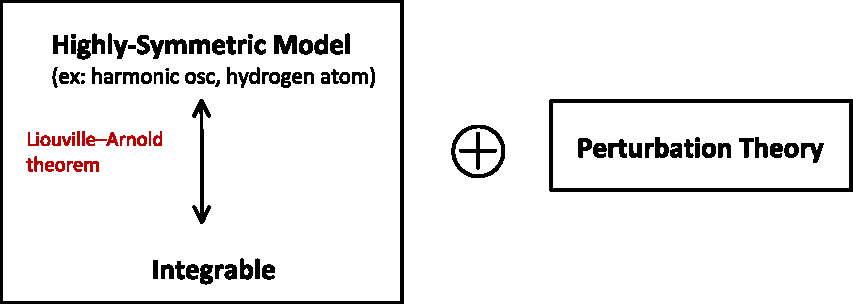
\includegraphics[width=1\textwidth]{images/General_Paradigm.pdf}
	\caption[General Paradigma]{General Paradigma. Integrable means that you can solve it up to computing integrals; it is a little bit weaker than solvable, solvable means that you can write a solution in terms of analytic functions.}
	\labfig{General Paradigma}
\end{figure}
So we explore the world of highly symmetric systems, which are solvable (or, at least, integrable\sidenote{\href{https://it.wikipedia.org/wiki/Teorema_di_Liouville-Arnold}{Liouville–Arnold theorem}\index{Liouville–Arnold theorem}:\\ In dynamical systems theory, the Liouville–Arnold theorem states that if, in a Hamiltonian dynamical system with $n$ degrees of freedom, there are also $n$ independent, Poisson commuting first integrals of motion, and the energy level set is compact, then there exists a canonical transformation to action-angle coordinates in which the transformed Hamiltonian is dependent only upon the action coordinates and the angle coordinates evolve linearly in time. \textbf{Thus the equations of motion for the system can be solved in quadratures} if the level simultaneous set conditions can be separated}), and thanks to perturbation theory we explore the family of models which are around them. In this course we touch only the books on the left hand side of the \reffig{General Paradigma}. Before talking about symmetries we have to talk about transformations.
\section{Transformations}
We are interested in two kind of transformations:
\[
\textrm{Transformations}
\begin{cases}
&\textrm{In the laboratory}\\
&\textrm{In the theory}
\end{cases}
\]
First, let us start in the laboratory where we suppose having a physical system, like a chair or an ammonium molecule. We always have to keep in mind that this system is not isolated in the universe, it is related to some measurement apparatus (in our scheme the Cartesian axes). Now we can perform a transformation $T$ on this setting (the 2D rotation\sidenote{\[ T =
\begin{bmatrix}
  \cos \theta & -\sin \theta\\
  \sin \theta &  \cos \theta
\end{bmatrix}\]}).
\begin{figure}[H]
	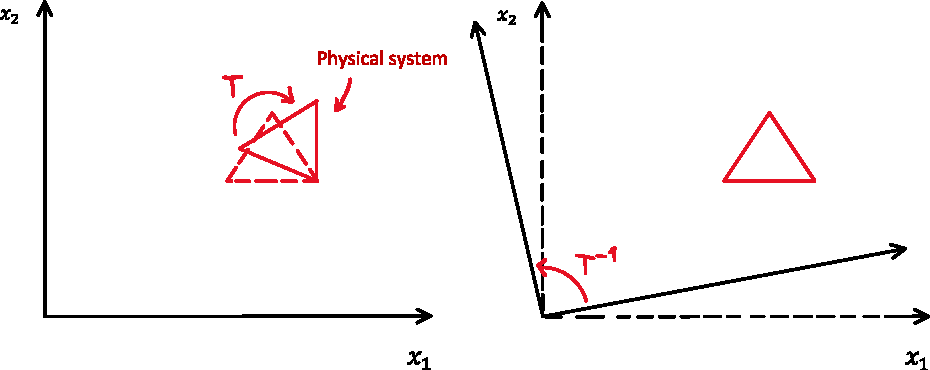
\includegraphics[width=1\textwidth]{images/Laboratory_scheme.pdf}
	\caption[Laboratory scheme]{Laboratory scheme to measure the position an ammonium molecule. It shows the two kind of transformation I can perform keeping the relative position the same.}
	\labfig{Laboratory scheme}
\end{figure}
\[
\textrm{\textbf{Active} transformation}\ \underset{\mathclap{\tikz \node {$\uparrow$} node [below=1ex] {\footnotesize We believe they should be equivalent};}}{\simeq}\ \textrm{\textbf{Passive} transformation}
\]
We call \index{Active transformation}\textit{active transformation} when the apparatus stay fixed. But maybe, we are not able to rotate the molecule and therefore we decide to rotate the measurement apparatus: we call this a \index{Passive transformation}\textit{passive transformation}. We believe that these two ways of approaching a transformation should be equivalent (i.e. experimentally indistinguishable), because we believe that the absolute position and absolute direction of physical system and apparatus are irrelevant. In fact, what is relevant is the \textbf{relative} position and orientation of the physical system \textit{with respect} to our apparatus.\sidenote{This is one of the funding principles of every theory, which will generalize in the \href{https://it.wikipedia.org/wiki/Principio_di_relativit\%C3\%A0}{principle of relativity}, but for now let us keep time frozen as specified in \vrefsec{Symmetry}}
\begin{assumption}[Principle of \textbf{homogeneity} and \textbf{isotropic} of space]\labass{Principle-of-homogeneity} The outcomes of any experiment does not depend on the \textbf{absolute position} and \textbf{orientation} of the system and the apparatus [it depends only on the \textbf{relative position}]
\end{assumption}
This transformation $T$ is something which lives in the laboratory, so it is really a physical transformation, therefore we want to describe it in our mathematical theory. Hence to the transformation $T$ are associated two mathematical object which are \textbf{dual} to each other:\sidenote{The space of states is connected to the Schrödinger representation, while the observable algebra to the Heisenberg representation.}
\begin{align*}
    S \xrightarrow{\hat{T}} S \quad \qquad  \qquad & \qquad \qquad \qquad \qquad A \xrightarrow{\tilde{T}} A\\
    S: \textrm{ space of states } \qquad & \qquad A: \textrm{ algebra of observable quantities}
\end{align*}
$\hat{T}$ is a \index{Map} map from the space of states to itself which represent the physical transformation $T$ in the mathematical theory. $\tilde{T}$ comes from $\hat{T}$, but it lives in the algebra of quantities.
\begin{enumerate}
    \item $\hat{T}$: rotation of the system;
    \item $\Tilde{T}$: rotation of the apparatus.
\end{enumerate}
Because of the \refass{Principle-of-homogeneity} we expect the two mathematical object to be related each other. Now we could ask who are these two object we have just introduced: this depends on the theory (for example: QED or classical mechanics), nevertheless we can elaborate a general structure.

\section[Structure of a.e. physical theory]{Structure of $\cancel{\textrm{any}}$ \textbf{a.e.} physical theory}
\marginnote{The word "any" is too ambitious. Better using "a.e." = "almost every", since some theories do not fit this framework, a remarkable example is \textbf{cosmology}. In this framework is needed a clear separation between the physical system and the investigation (the laboratory), while in cosmology the apparatus is part of the system.}The professor's personal view point is that a physical theory is essentially a relation between what happens in the laboratory and what happens in the world of mathematics, mediated by some rules.
\marginnote[40 mm]{Outcomes = Statistical distribution of outcomes in $N$ repetitions of a single experiment.}
\marginnote[72 mm]{For example in Q.M: orthogonal projector have eigenvalue $0$ or $1$.}
\marginnote[120 mm]{What to put in the boxes on this part of the diagram depends on the theory we are looking at.}
\begin{figure}[H]
	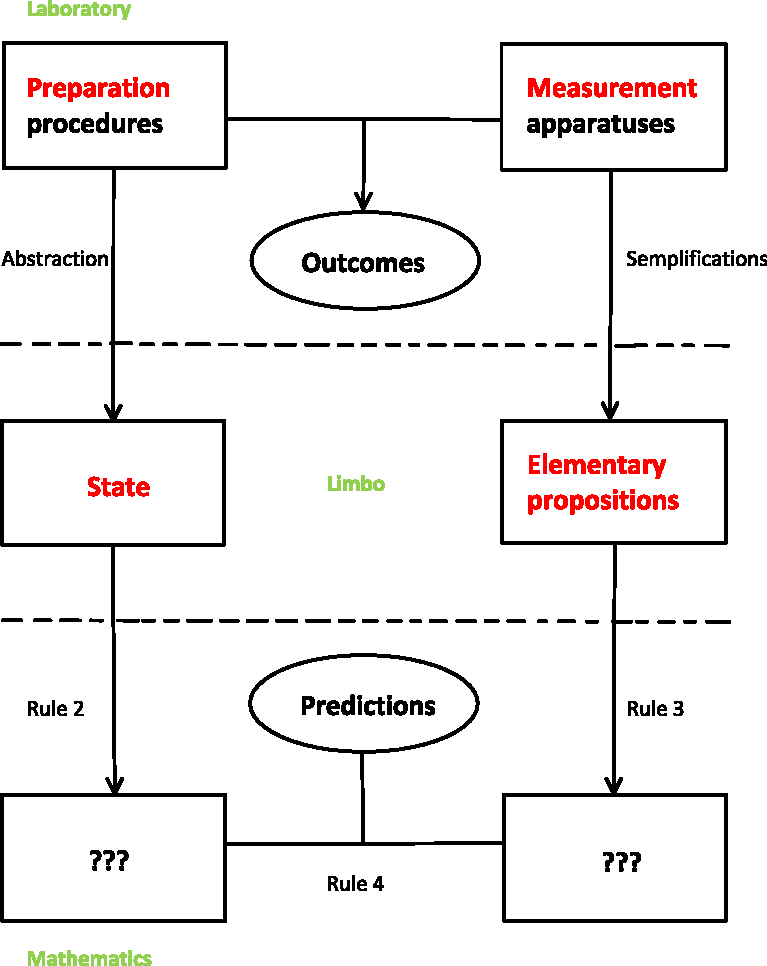
\includegraphics[width=1\textwidth]{images/Schema_Phys_theory.pdf}
	\caption[Schema Physical Theory]{Scheme of a physical theory.}
	\labfig{Schema Phys Theory}
\end{figure}
\begin{itemize}
    \item \textbf{Laboratory:} at this level there are two fundamental boxes.
    \begin{itemize}
        \item \index{Preparation procedure}Preparation procedure: a concrete series of operation to perform on the system to prepare it to the measurement.\sidenote{For example: take a glass of water, bring it to 72°, wait 3', insert an electric field of some intensity and then we will measure some properties.}
        \item \index{Measurement apparatuses}Measurement apparatuses.
    \end{itemize}
    If we combine the two we will obtain some numbers which are the outcomes of the measurement, which depend on the two boxes.
    \item \textbf{Limbo:} Where we do some abstraction procedure, before translating our concept in the world of mathematics, since wee cannot hope to really have a general description\sidenote{Because every laboratory is different from every other and so are the measurements.}. Here we find two concepts:
    \begin{itemize}
        \item \index{State}State: we will discuss it later.
        \item \index{Elementary propositions/experiment}Elementary propositions/experiment: instead of considering all the possible measurement apparatuses, we will restrict, namely, to those experiment in which the possibles answers are only \textit{yes} (1) and \textit{no} (0).\sidenote{Instead of asking the position of the electron, which answer will be the three coordinates in a classical theory, we will ask ourselves: << Given a box $\Omega$ is the electron detected in this box? >>} This correspond in quantum mechanics to \index{Orthogonal projectors} \textit{orthogonal projectors}, whose eigenvalue are only $0$ and $1$.
    \end{itemize}
    Maybe we will not have time to do that, but one can prove that if we know the answer to all the possible elementary propositions (orthogonal projectors) in any state of the system, we will be able to reconstruct the answer to any other experiment (observable quantity).
    \item \textbf{Mathematics}: Here we will have two boxes that are theory-dependent: one which corresponds to the "Preparation procedures" and one which corresponds to the "Measurement apparatuses". The combinations of these two mathematical objects we will give us some numbers, which are our predictions.
\end{itemize}
Our theory is successful if the predictions agree with the outcomes of our experiments, within a reasonable error/accuracy.
\section{States of a physical system}
The notion of state as a system is so common in classical mechanics that it entered quantum mechanics without any reflection, but it useful to reflect on that to understand what is the state of a system.
\subsection[State in Classic Mechanics]{State in classical mechanics (CM)}
We know that in classical mechanics
\begin{definition}[State in classical mechanics]
A state of the system is the set of all the positions and the momenta of the particle which the system consist of as a state.
\end{definition}\labdef{state-classical}
\begin{figure}[H]
	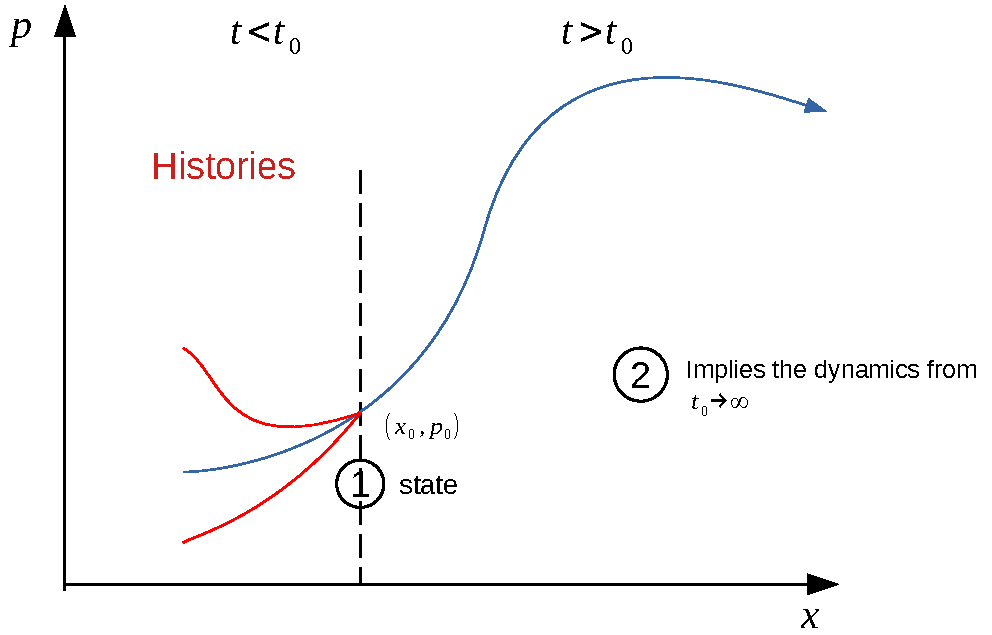
\includegraphics[width=1\textwidth]{images/spazio_fasi_classico.pdf}
	\caption[Classical phase space]{Classical phase space for a particle. Note that before $t_0$ there would be just one line if we were able to describe the dynamics with an Hamiltonian. But since the system is not autonomous (because it is in relation with the laboratory) this is not possible.}
	\labfig{Classical Phase Space}
\end{figure}
\begin{example}
The state space of a single classical particle in $\mathbb{R}^d$ are the pair:\marginnote{We use the mathematical notation convection: \[x = \left(x_1,\dots,x_d\right)\in\mathbb{R}^d\] \[p = \left(p_1,\dots,p_d\right)\in\mathbb{R}^d\]}
\[
S=\mathbb{R}^d\times \hat{\mathbb{R}}^d \ni \left(x,p\right)
\]
where $p$ is the momentum\footnote{We use the $\wedge$ symbol because it reminds the Fourier transform.}.
\end{example}
Let us reflect on what does it mean. In a sense it means that if we know position and momentum/velocity of the particle at the same time, in CM we know the solution forever\sidenote{The Newton equation is a II order equation, knowing the initial condition (position and velocity) the Cauchy problem associated is resolved for all $t$}. Looking at the phase space, the knowledge of the initial states implies the dynamics from the time our system starts $t_0$ up to infinity. So we could rephrase the classical definition of state with the following:
\begin{definition}[State in classical mechanics according to information theory\index{Information theory}]
A state of the system is the amount of information which is needed to predict the future dynamics of the system.
\end{definition}\labdef{state-classical}
But we could also look at the picture from another view point and say that if the dynamics is Hamiltonian, there is only one trajectory which passes through the point $(x_0,p_0)$. Let us suppose this to be false, it means that there could be different procedures that bring us to the same position and momentum. We could say that all the histories before $t_0$ are equivalent, in the sense that the behaviour of the system after $t_0$ does not depend on the particular history/preparation procedure. This is a good view point that we can incorporate in a quantum theory.

\subsection{States in a general theory}
\begin{definition}[pseudo definition - single particle in $\mathbb{R}^d$]
A \textbf{state} is an \textbf{equivalence class of preparation procedures} where two procedures are considered  equivalent if they differ by \textbf{\underline{irrelevant} details.}
\end{definition}
\marginnote{There is a bit of tautology in this definition. We all agree that the color of the wall of the laboratory is not an essential detail as well as the color of the clothes of the experimentals, but the altitude of the laboratory? It depends on the experiment you are performing.}
The trick of this definition which makes it a pseudo one is that you do not a priori what is relevant.
\begin{kaobox}[frametitle=Remark]
Relevance or irrelevance is decided a posteriori: details are not relevant if they do not reflect on the outcomes of the experiment.
\end{kaobox}
We have defined a state in the \textit{limbo} (i.e. an equivalent class of the preparation procedure), then we decide to associate to it some mathematical object and this will be theory dependent.
\section[Structure of CM]{Structure of Classical Mechanics}
\marginnote{Structure = states + observables\\ Set = "Insieme" in Italian.}
As before, to simply, let us take just one particle
\[
\textrm{State: } \quad S = \mathbb{R}^d \times \hat{\mathbb{R}} \ni \left(x,p\right)
\]
In the theory of classical mechanics the elementary propositions are represented by taking a characteristic function of a subset of our phase space\sidenote{We are using the notation of quantum mechanics even if is a classical theory to show the analogy}:
\begin{align*}
    \textrm{Elementary propositions: }& \textrm{Characteristic function of a set } \Omega \subseteq \mathbb{R}^d\times\hat{\mathbb{R}}^d\\
    & \chi_{\Omega}(x,p) = \begin{cases}
    0 \quad \textrm{if} \ (x,p) \notin \Omega\\
    1 \quad \textrm{if} \ (x,p) \in \Omega
    \end{cases}
\end{align*}
\begin{marginfigure}
	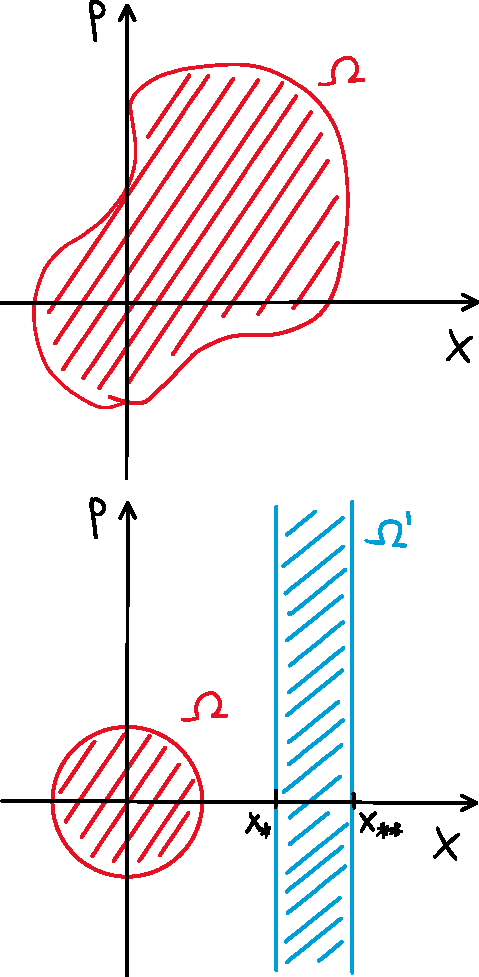
\includegraphics{images/subset_class_mech.pdf}
	\caption[Examples of subset in CM]{Examples of subsets in classical mechanics. The red ones mix position and momentum, while the blue one leave the momentum free.}
	\labfig{subset-class-mech}
\end{marginfigure}
And then the coupling is
\[
    \textrm{Coupling for elem. prop.: } \quad \expval{\chi_\Omega}_S= \chi_\Omega(s) = \begin{cases}
    0 \quad \textrm{if} \ s \notin \Omega\\
    1 \quad \textrm{if} \ s \in \Omega
    \end{cases}
\]
The observables are not all elementary propositions, since we can generate any reasonable function. For example the general function will be any continuous function over the phase space, they can be generated as linear combination and limit\footnote{We are not covering the details to justify this sentence.}
\[
    \textrm{Observables: } \quad A=C(s) = C\left(\mathbb{R}^d\times\hat{\mathbb{R}}^d\right) \quad \leftarrow\textrm{$\mathbb{R}$ valued functions}
\]
There are many relevant elements
\begin{enumerate}
    \item Total energy: \(H(x,p)=\frac{1}{2m}p^2+V(x)\)
    \item First component of angular mom.: \(L_1(x,p)=x_2p_3-x_3p_2\)
    \item Every other continuous function: F(x,p)
\end{enumerate}
The coupling between general observable and (\textit{miss}) states is
\[
    \textrm{\underline{Coupling}: } \quad \expval{F}_S= F(s)\in\mathbb{R}
\]
\section[Structure of QM]{Structure of Quantum Mechanics}\marginnote[10mm]{We will use this notation:
\begin{enumerate}
    \item \textbf{Quantum mechanics}: we will intend the quantum theory of a finite number of particle, or a quantum system with finally many degrees of freedom.
    \item \textbf{Quantum field theory}:the theory of a quantum system with infinitely many degrees of freedom.
    \item \textbf{Quantum theory:} everything, i.e. QM, QFT, etc...
\end{enumerate} }
The first part of the diagram \vreffig{Schema Phys Theory} is theory independent. Now we have to give rules to associate which associate a state to an object in our mathematical world (similarly also elementary propositions) to get numbers (expectation values).
\begin{definition}[\underline{State} in quantum mechanics]
A state in QM is represented by a \textbf{ray} in a (separable, complex)\footnote{We will omit this specification further on} Hilbert space. A ray is\footnote{If the ray is the zero vector it is not normalizable and we are lost.}
\[
\textrm{if} \quad \psi \in \pazocal{H}, \quad \psi \neq 0
\]
therefore the ray can also be seen as the span and use the following notation
\[
\qty[\psi] = \left\{\lambda \psi : \ \lambda\in\mathbb{C}\right \} = \left\{\omega \frac{\psi}{\norm{\psi}} : \ \omega \in U(1)\right \}
\]
where $U(1)$ is the unit sphere: \ \( U(1) = \left\{z\in\mathbb{C} : \ \abs{z}=1\right\}\).
\end{definition}\labdef{state-in-qm}
\begin{kaobox}[frametitle=Nota]
The intersection of a ray with the unite sphere happens in two circles: one around $\psi$ and the other around $-\psi$. Circles and not points because of the inner phase.
\end{kaobox}
\begin{marginfigure}
	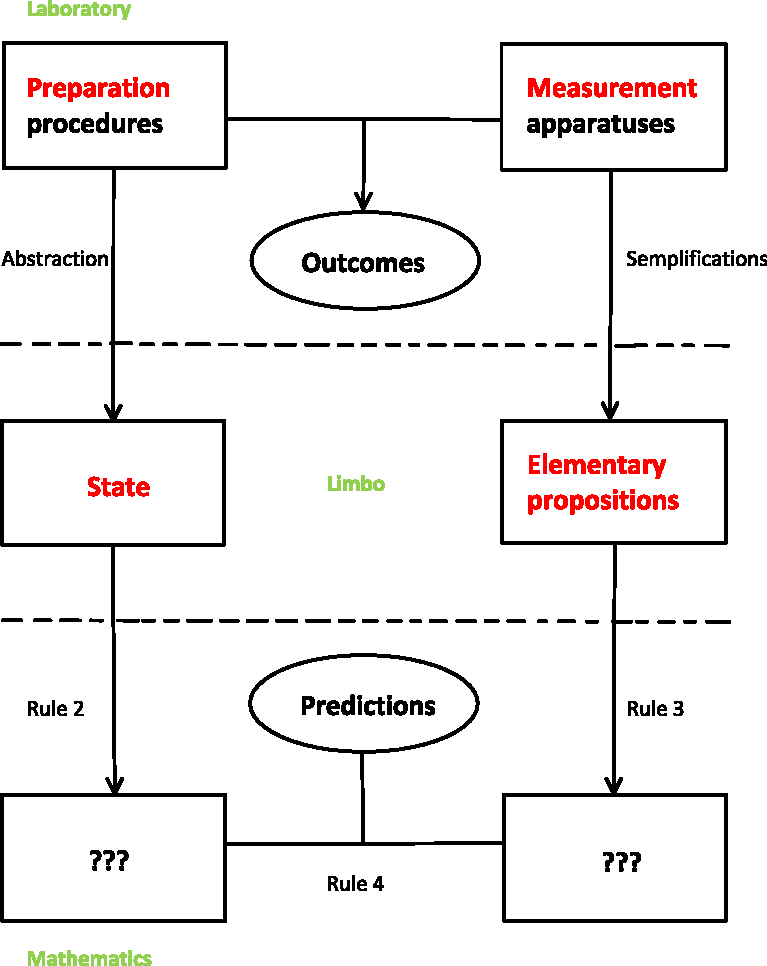
\includegraphics[width=1.1\linewidth]{images/Schema_Phys_theory.pdf}
	\caption[Schema Phys theory small]{Re-proposing of the previous scheme.}
	\labfig{Schema_Phys_theory2}
\end{marginfigure}
For many applications the distinction between ray and vector makes no difference, but for this course it is important that a state in a quantum mechanical theory is represented by a ray and not by a vector, because the phase ambiguity plays a crucial role in the second part of the course. Therefore $\qty[\psi]$ is the equivalence class (the family) of all the vectors which difference from $\psi$ by a complex phase.
\begin{figure}[H]
	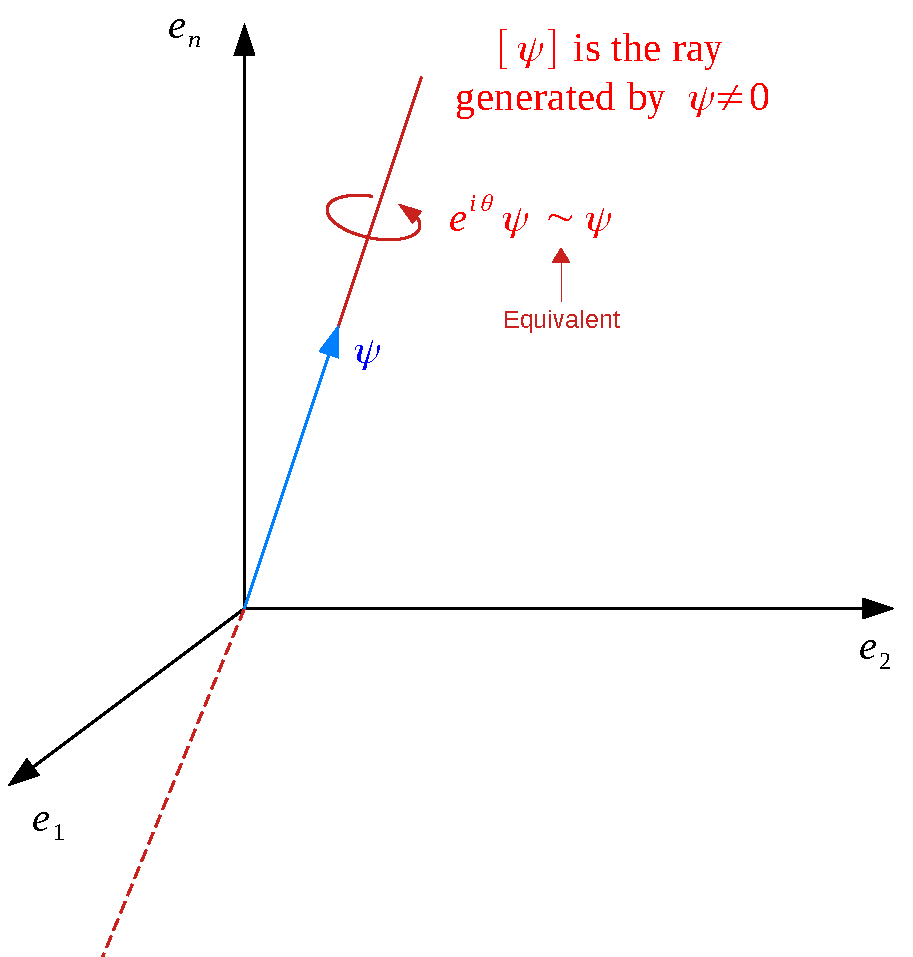
\includegraphics[width=1\textwidth]{images/State_QM.pdf}
	\caption[Rep. of a state in QM]{Representation of a ray in just three directions.
	\begin{enumerate}
	    \item A state vector in any non zero vector.
	    \item The ray is two dimensional because it is made of complex numbers.
	\end{enumerate}}
	\labfig{Rep-state-QM}
\end{figure}
Mathematicians like to give a name to this space
\begin{definition}[Projective space]
\index{Projective space}: It is the space of rays in a Hilbert space
\[
\mathbb{P}\pazocal{H} = \left\{\psi \in \pazocal{H}: \psi \neq 0\right\}\big/ \underset{\mathclap{\tikz \node {$\uparrow$} node [below=1ex] {\footnotesize Equivalent relations};}}{\sim}
\]
where I divided with respect to an \index{Equivalent relation}equivalent relations that identifies points which are equivalent, i.e. an equivalent relation is\marginnote{$\mathbb{C}^*$ means $\mathbb{C}\setminus\{0\}$}
\[
\psi \sim \tilde{\psi}:\  \exists\  \lambda \in \mathbb{C}^*:\ \tilde{\psi} = \lambda\psi
\]
\end{definition}
While the elementary propositions and the coupling are represented by:\marginnote{The expectation value is a real number because it is self-adjoint}
\begin{align*}
    \textrm{Elementary propositions: }& \textrm{Orthogonal projections } \ E\in B(\pazocal{H})\\
    & E^2=E=E^*
\end{align*}
\[
    \textrm{\underline{coupling}: } \expval{E}_\qty[\psi]=\braket{\psi}{E\psi}\in\mathbb{R} \quad \quad \star
\]
The difference with classical mechanics is that now the expectation values are not only $0$ and $1$, but in general it will have component in both directions/subspecies (unless $\psi$ is an eigenvector of $E$). Now the predictions have a statistical structure. So even if in a single experiment the elementary propositions can be measured only either \textit{True} or \textit{False}, the prediction of the theory is a number between $0$ and $1$, which is the expectation value on average after $N$ repetitions.
\begin{kaobox}[frametitle=Notation]
Hereafter we denote the inner product\index{Inner product} in $\pazocal{H}$ by the symbol $\braket{\dots}$ (the \href{https://it.wikipedia.org/wiki/Notazione_bra-ket}{Dirac bra-ket notation}), so that
\[
\braket{\psi}{\varphi}=\overline{\braket{\psi}{\varphi}}
\]
We always assume that $\braket{\dots}$ is \textbf{antilinear} with respect to (w.r.t.) the first variable (as in the Physics textbook).\marginnote[-10mm]{Although in Physics, by definition $A$ is applied on the right in the Dirac's notation; Panati, probably influenced by the mathematical notation, quits this ambiguity by writing explicitly if the operator $A$ acts on the ket or on the bra:
\[
\left(\mathbf{v}, A\mathbf{w}\right)\equiv \bra{v}\ket{Aw} \underset{\mathclap{\tikz \node {$\uparrow$} node [below=1ex] {\footnotesize Dirac's notation};}}{=} \bra{v}A\ket{w}
\]}

\end{kaobox}
A general observable will be represented by a bounded operator $A\in B_{\textrm{\textbf{sa}}}(x)$ such that $A^*=A$ (self-adjointed). This is nothing new, it follows from the previous one. We can convice ourselfs looking at the example on the \reffig{obs-quant}
\begin{figure}[H]
	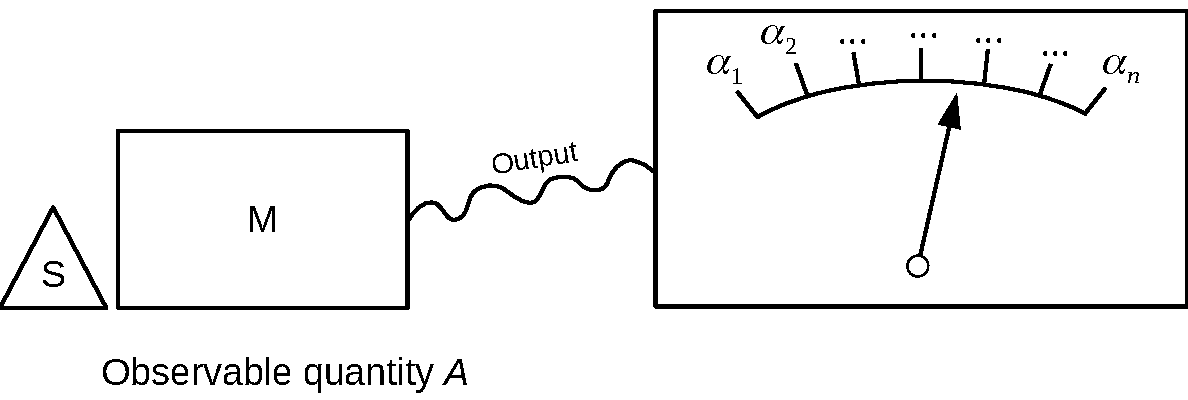
\includegraphics{images/strumento_misura_osservabile.pdf}
	\caption[Apparatus to measure a quantity]{Example of a physical system (S) which produces an observable $A$ that interact with the measurement apparatus M. The latter will produce a macroscopic output that at the very end of the experiment will make the pointer point on some outcome.}
	\labfig{obs-quant}
\end{figure}
ince our apparatus has a finite scale with finite accuracy, we will have a finite number of possible values $\alpha_i$. 
Now consider this yes/no experiment
\[
\begin{split}
\textrm{Elementary proposition: } &e_j = \textrm{"the pointer is measured in the j-th position"}\\
&\big\updownarrow\\
& E_j = E_j^2=E_j^\ast
\end{split}
\]
But this might no be enough, we must assume to have a classical measurement apparatus
\begin{assumption}[\textbf{Classicality} of measurament apparatus]\labass{class-meas-app} The pointer cannot be measured in a superposition of the $j$-th and the $l$-th position if $j\neq l$. Mathematically it means that the projectors $\begin{Bmatrix}
  \hat{E}_j
\end{Bmatrix}_{j=1}^n$ associated with the elementary proposition $e_j$ are \textbf{mutually orthogonal}, this means that
\begin{align*}
\hat{E}_j\hat{E}_l=
\begin{Bmatrix}
\hat{E}_j & \mbox{if } j=l\\
0 & \mbox{if } j\ne l
\end{Bmatrix}=\delta_{jl}\hat{E}_j
\end{align*}
\end{assumption}
This is enough to conclude that the expectation value of the observable $A$ can be described statistically by a self adjointed operator. In fact, we are now able to compute the mean value and the variance of an observable $A$ over a state $\psi$. Suppose we are measuring an energy:\marginnote{We demonstrate in the course of \href{https://www.overleaf.com/read/hczjjtmcwsvj}{QM (pag 50-51)} in the bachelor that \[
\ev{\hat\xi}{\psi}=\sum_{i}\xi_i\textrm{Prob}\left(\xi_i\textrm{ su }\ket{\psi}\right)
\]}
\begin{align*}
\langle A \rangle _{\psi}=\sum_{j=1}^n \alpha_j \textrm{p}(e_j \mbox{ is true})=\sum_{j=1}^n \alpha_j \langle \psi | \hat{E}_j \psi \rangle=\langle \psi | \underbrace{\left(\sum_{j=1}^n \alpha_j \hat{E}_j\right)}_{\textrm{We call this operator } A}\psi \rangle 
\end{align*}
\marginnote{Recall of the course of QM
\begin{postulato}\labpost{operatore_osservabile}
\textbf{Operatore $\hat{\xi}$ associato a un osservabile $\xi$}\index{Operatore}\footnote{Questo postulato è indicato come \href{https://it.wikipedia.org/wiki/Postulati_della_meccanica_quantistica\#Le_osservabili}{Le osservabili} su Wikipedia.}\\
Scelta una base ortonormale di autovettori $\ket{\xi_i}$ dell'osservabile $\xi$, si associa un operatore $\hat{\xi}$ autoaggiunto su $\pazocal{H}$ definendolo sui vettori di questa base come:
\[
\hat{\xi}\ket{\xi_i^{\left(\alpha\right)}}\overset{\textrm{def}}{=}\xi_i\ket{\xi_i^{\left(\alpha\right)}}
\]
\end{postulato}
Possiamo quindi estendere questa definizione su uno stato generico $\ket{A}$ per linearità:
\[
\begin{split}
\hat{\xi}\ket{A}\overset{\mathclap{\tikz \node {↓} node [above=1ex] {\footnotesize $\ket{\xi_i^{\left(\alpha\right)}}$ base};}}{=}\hat{\xi}\left(\sum_{i\alpha}\ket{\xi_i^{\left(\alpha\right)}}a_{i\alpha}\right)
&\overset{\textrm{def}}{=}\sum_{i\alpha}a_{i\alpha}\hat{\xi}\ket{\xi_i^{\left(\alpha\right)}}\\
&\underset{\mathclap{\tikz \node {$\uparrow$} node [below=1ex] {\footnotesize \refpost{operatore_osservabile}};}}{=} \sum_{i\alpha}a_{i\alpha}\xi_i\ket{\xi_i^{\left(\alpha\right)}}
\end{split}
\]
}We notice that, since $\alpha_j$ is real:
\begin{align*}
    A\overset{\textrm{def}}{=}\sum_{j=1}^n \alpha_j E_j=\sum_{j=1}^n \alpha_j E_j^*=\left(\sum_{j=1}^n \alpha_j E_j\right)^*=A^*
\end{align*}
Up to this point, we did not use the \refass{class-meas-app}. To define the variance instead:
\begin{align*}
    \textrm{Var}(A)_{\psi}
    &=\sum_{j=1}^n\left(\alpha_j-\langle A \rangle_{\psi}\right)^2p(e_j \mbox{ is true})=\\
    &=\sum_{j=1}^n\alpha_j^2\langle \psi|E_j \psi \rangle - \langle A \rangle_{\psi}^2=\\
    &=\langle \psi|\sum_{j=1}^n\alpha_j^2E_j \psi \rangle - \langle A \rangle_{\psi}^2=\\
    &=\langle \psi|B \psi \rangle - \langle \psi|A \psi \rangle^2
\end{align*}
But we notice that, with the assumption \refass{class-meas-app}, we can express $A^2$ as:
\begin{align*}
    A^2
    =\left(\sum_{j=1}^n \alpha_j E_j \right)\left(\sum_{k=1}^n \alpha_k E_k \right)
    =\sum_{j,k=1}^n\alpha_j\alpha_k {\color{red} E_jE_k}\overset{\mathclap{\tikz \node {↓} node [above=1ex] {\footnotesize \color{red} $E_jE_k=\delta_{jk}E_j$};}}{=}
    \sum_{j,k=1}^n\alpha_j\alpha_k\delta_{jk}E_k
    =\sum_{j=1}^n\alpha_j^2 E_j
    =B
\end{align*}
Therefore we found the usual rule of Quantum Mechanics
\[
\textrm{Var}(A)_\psi= \langle \psi|A^2 \psi \rangle - \langle \psi|A \psi \rangle^2
\]
It would have been very inconvenient if we had to add another operator to describe the variance and then other operators to describe the higher order moments of the statistical distribution. The \refass{class-meas-app} allows us to use the same operator, instead of defining the operator $B=\sum_{j=1}^n\alpha_j^2E_j$ for the variance. We will not demonstrate that other powers of the operator $A$ would be sufficient for the other momenta.
\section[Transformation in CM]{Transformation in classical mechanics (CM)}
Let's suppose to have a simple particle in $\mathbb{R}^d$, we already discussed the state $(x,v)\in S=\mathbb{R}^d\times \hat{\mathbb{R}}^d$. Suppose that in the laboratory there is concrete linear physical transformation $T: \mathbb{R}^d\to\mathbb{R}^d$. From this one we have to define the two related object:\marginnote{If we used the momentum $p$ instead of the velocity we should have use the transposed of $T$ for the transformation.}
%39:00
\begin{align*}
\hat{T}: S \rightarrow S \, \mbox{ such that } \, \hat{T}(x,v)=(Tx,Tv)
\end{align*}
and $\tilde{T}(F)$ with $\tilde{T}:A \rightarrow A$, where $A_{\textrm{cl}}=C(\mathbb{R}^d\times\hat{\mathbb{R}}^d)$. By the principle of \textbf{homogeneity} and \textbf{isotropy} of space (\vrefass{Principle-of-homogeneity}) , we know that $\forall \ F \in A_{\textrm{cl}} \quad \forall \ s \in S$ \marginnote{$\langle \tilde{T}(F) \rangle_{\hat{T}(S)}$ means the expectation value of the rotate observable in the rotated state.}
\[
\star \quad \langle \tilde{T}(F) \rangle_{\hat{T}(S)}=\langle F \rangle_S \ \Rightarrow \ \tilde{T}(F)(Tx,Tv)=F(x,v) \quad \forall (x,v)\in S
\]
therefore, by a change of variable, we obtain $$\tilde{T}(F)(x,v)=F(T^{-1}x,T^{-1}v) \quad \forall (x,v)\in S \quad \star$$
\begin{kaobox}[frametitle=Moral]
The form of $\tilde{T}:A_{\textrm{cl}} \xrightarrow[]{} A_{\textrm{cl}}$ \, is prescribed once we give the transformation of the state $\hat{T}:S \rightarrow S$ and assume the \refass{Principle-of-homogeneity}\footnote{In the last chapter it will be the principle of relativity.}.
\end{kaobox}
\section[Transformation in QM]{Transformation in quantum mechanics (QM)}\marginnote{This part is treated in detail in Chapter ???.}
Let's suppose to have a simple particle in $\mathbb{R}^d$, an Hilbert space $\pazocal{H}=L^2(\mathbb{R}^d,dx)$, where $L^2$ denotes the class of square integrable functions\sidenote{The \href{https://it.wikipedia.org/wiki/Funzione_a_quadrato_sommabile}{square integrable functions} are functions $\psi:\mathbb{R}^d\rightarrow\mathbb{C}$ such that \[\int_{\mathbb{R}^d}\abs{\psi}^2dx< +\infty\]The vector space of square integrable functions (with respect to Lebesgue measure) forms the $L^p$ space with $p = 2$. Among the $L^p$ spaces, the class of square integrable functions is unique in being compatible with an inner product, which allows notions like angle and orthogonality to be defined. Along with this inner product, the square integrable functions form a Hilbert space, since all of the $L^p$ spaces are complete under their respective p-norms.}, and the state space $S=\mathbb{P}(\pazocal{H})$ is a set of \textbf{rays in the Hilbert space} $\pazocal{H}$. To our concrete transformation $T$, we should associate $\hat{T}:S \rightarrow S$ such that it preserves the structure of our projective space. Spoiler: the Wigner's theorem states that every automorphism of the state space $S=\mathbb{P}(\pazocal{H})$, i.e. every transformation of $S$ which preserves the structure of $S$, is generated either by a \textbf{unitary} \underline{\underline{or}} \textbf{anti-unitary} operator, by setting
\[
\hat{T}\qty[\psi]=\qty[U\psi]
\]
(if $\psi\neq 0$ also $U\psi\neq 0$) so it gives a ray.
\begin{definition}[Unitary operator]\index{Unitary operator}
A unitary operator $U:\pazocal{H}\rightarrow\pazocal{H}$ is a linear operator such that
    \begin{enumerate}
        \item preserves the inner product: $\langle U\psi|U\varphi \rangle=\langle \psi|\varphi \rangle \quad \forall\ \psi,\varphi \in \pazocal{H}$
        \item it is \textbf{surjective}\footnote{In finite dimension this condition is automatic.}:  $\textrm{Ran}U=\pazocal{H}$
    \end{enumerate}
\end{definition}
\begin{kaobox}[frametitle=Remarks]
From 1. it follows that $U$ preserves the norm:
$$||U\psi||^2=\langle U\psi|U\psi \rangle=\langle \psi|\psi \rangle=||\psi||^2$$
Therefore, $U$ is an \textbf{isometry}\index{Isometry}, i.e. it preserves lenght, and it is also \textbf{injective} \cite{abate2006geometria}\marginnote[-25mm]{
From \cite{abate2006geometria} pag 97-98:\\
\textbf{Poposizione}: Sia $T:V\to W$ un'applicazione lineare. Allora $T$ è iniettiva se e solo se Ker$T=\{O\}$.
\begin{proof}
Se $T$ è iniettiva, $T(v)=O=T(O)$ implica $v=O$ e quindi Ket$T=\{O\}$. Viceversa, supponiamo Ker$T=\{O\}$. Prendiamo $v_1$, $v_2\in V$ tali che $T(v_1)=T(v_2)$; dobbiamo dimostrare che $v_1=v_2$. Ma $T(v_1)=T(v_2)$ equivale a  $T(v_1)-T(v_2)=O$, da cui segue $T(v_1-v_2)=O$ e dunque $v_1-v_2=O$, dove l'ultima implicaziomne vale in quanto Ker$T=\{O\}$.
\end{proof}

From \cite{abate2006geometria} page 100 \\
\textbf{Corollario}: Sia $T:V\to W$ un'applicazione lineare. Allora:
\begin{enumerate}
    \item $T$ è iniettiva se e solo se rg$T$=dim$V$;
    \item $T$ è surgettiva se e solo se rg$T$=dim$W$;
    \item se dim$V$ = dim$W$ (in particolare, se $V=W$), $T$ è iniettiva se e solo se è surgettiva.
\end{enumerate}
\begin{proof}
\begin{enumerate}
    \item L'applicazione $T$ è iniettiva se e solo se Ker$T=\{O\}$, ovvero se e solo se si ha sim Ket$T=0$; basta allora applicare il "Teorema della dimensione".
    \item $T$ è surgettiva se e solo se Im$T=W$, che  può succedere se e solo se rg$T$=dim$W$ (altra Prop.).
    \item Basta confrontare 1. e 2..
\end{enumerate}
\end{proof}
}:
$$\mbox{ker }U=\begin{Bmatrix}\psi\in\pazocal{H}:U\psi=0\end{Bmatrix}=\begin{Bmatrix}\psi\in\pazocal{H}:||\psi||=0\end{Bmatrix}=\begin{Bmatrix} O\end{Bmatrix}$$
If $\pazocal{H}\cong\mathbb{C}^N$, it happens $U:\mathbb{C}^N\xrightarrow[]{}\mathbb{C}^N$ then, for a linear map, \textbf{injectivity} \underline{implies} \textbf{surjectivity} in finite dimensions.
\end{kaobox}
\begin{definition}[\textbf{Anti}-unitary operator]\index{Anti-unitary operator}
An anti-unitary operator\\ $T:\pazocal{H}\xrightarrow[]{}\pazocal{H}$ is an \textbf{anti}-linear operator, i.e.
        \(
        \forall \ \lambda \in \mathbb{C} \quad T(\lambda\psi)=\Bar{\lambda}T(\psi)
        \), with $\Bar{\lambda}$ the complex conjugate of $\lambda$, such that:
    \begin{enumerate}
        \item 
        \[\langle T\varphi|T\psi \rangle=\overline{\langle \varphi|\psi \rangle}\underset{\mathclap{\tikz \node {$\uparrow$} node [below=1ex] {\footnotesize by hermitianity of the inn. prod.};}}{=}\langle \psi|\varphi \rangle\]
        \item It is surjective
    \end{enumerate}
\end{definition}
\begin{example}
Spinless particle in $\mathbb{R}^d$.\\
In this case the Hilbert space is $\pazocal{H}=L^2(\mathbb{R}^d,dx)$ and there is privileged anti-unitary operator: 
\[
\begin{split}
\mbox{complex conjugation }\  C:L^2(\mathbb{R}^d)&\xrightarrow[]{}L^2(\mathbb{R}^d)\\
\psi &\mapsto \Bar{\psi}
\end{split}
\]
$C$ is \textbf{antiunitry} and $C^2=+\mathbb{1}.$
\end{example}
%01:01:00
\begin{example}
Spin 1/2 particle in $\mathbb{R}^d$\\
In this case the Hilbert space is \[\pazocal{H}=L^2(\underbrace{\mathbb{R}^d,\mathbb{C}^2}_\text{\parbox{1.5cm}{\centering$\mathbb{C}^2$-valued\\[-4pt]  wave funct.s}})=L^2(\mathbb{R}^d)\otimes \mathbb{C}^2\]
An anti-unitary operator is the
\[
\mbox{Time-reversal operator}\ \Theta=C \otimes M
\]
where $C$ is the complex conjugation and $M$ the exponential of a Pauli matrix: $M=e^{-i\pi S_y/\hslash}$, with $(S_x,S_y,S_z)$ spin operators.
\end{example}
\section{Symmetry}\labsec{Symmetry}
\begin{kaobox}[frametitle=Terminology $\star$]
A \textbf{symmetry}\index{Symmetry} of a physical system is a transformation which leaves invariant the \textbf{generator of the dynamics}, i.e. the Hamiltonian (a function in CM, an operator in QM). For $\pazocal{H}\in A$, the transformation $\Tilde{T}(\pazocal{H})=\pazocal{H}$ is a symmetry of the system.
\end{kaobox}
We can do many transformations to our system, but it is not obvious that this will leave invariant the Hamiltonian.\sidenote{Rotating an ammonium molecule will not change anything, but squishing it do change the physics.} Not every transformation leaves invariant the dynamics. Sometimes we will call symmetries any transformation, but we will be wise enough to understand what it means by the context.
\begin{kaobox}[frametitle=Remark]
We are considering here a \textbf{non-Lorentz-invariant} (or covariant) approach, as we are assuming the existence of a distinguished \textbf{time axis}, so that the dynamics in QM is given by
\[
U(t) = e^{-i\frac{t}{\hslash}H} \quad \quad \left(t\in\mathbb{R}\right)
\]
with $\pazocal{H}$ the Hamiltonian operator.
\end{kaobox}
In the last chapter (Ch. 7) we will consider \textbf{relativistic theories} and we will adapt our approach accordingly. Equation (Symm) will be replaced by the \textbf{invariant of the action functional $S\qty{\phi}$}, where $\phi$ denote the relativistic field(s).
\section{Exercises}
There are no suggested exercises for this chapter, Just review the related concept from Geometry 1 and \href{https://www.overleaf.com/read/hczjjtmcwsvj}{Quantum Mechanics}.
\newpage
\vspace*{\fill} 
\begin{quote} 
{\centering 
Citation of the day:\\
"Prima non datur, ultima non dispensatur"}\\
\newline
Free translation: The first lecture is just an overview, the last one should not be missed.
\end{quote}
\vspace*{\fill}
\end{document}